\section{Discussion}

\paragraph{Goal}
In this paper I set up a goal to investigate if including pretext task in training process could reduce NNs
vulnerability against adversarial attacks.

\paragraph{Observations}
\begin{itemize}
    \item both pretext task reduced miss-classification rate a little
    \item both pretext task have improved accuracy a little
    \item both pretext tasks increased $\epsilon$ a little
    \item accuracy, miss rate, $epsilon$ are still far from competing with the values for EffNet pre-trained on ImageNet
\end{itemize}

\paragraph{Interpretation}


\begin{figure}[h]
    \begin{subfigure}{0.4\textwidth}
        \caption{Adversarial pattern \\ with no pretext task}
        \centering
        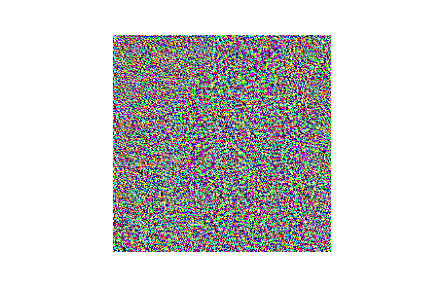
\includegraphics[width=8cm]{images/sunflower_adv_pattern}
    \end{subfigure}
    \begin{subfigure}{0.4\textwidth}
        \caption{Adversariual pattern \\ with rotation pretext task}
        \centering
        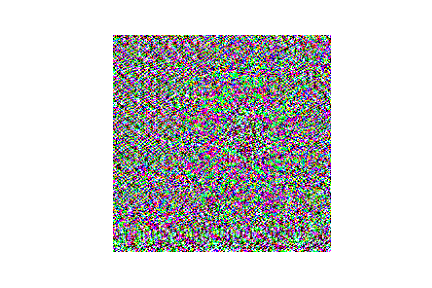
\includegraphics[width=8cm]{images/sunflowers_pr_adv_pattern}
    \end{subfigure}
    \\
    \begin{subfigure}{0.4\textwidth}
        \caption{Adversarial image \\ with no pretext task \\ $\epsilon$ = 0.1}
        \centering
        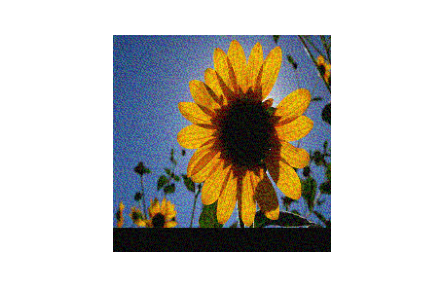
\includegraphics[width=8cm]{images/sunflower_adv_attack_01}
    \end{subfigure}
    \begin{subfigure}{0.4\textwidth}
        \caption{Adversariual pattern \\ with rotation pretext task \\ $\epsilon$ = 0.1}
        \centering
        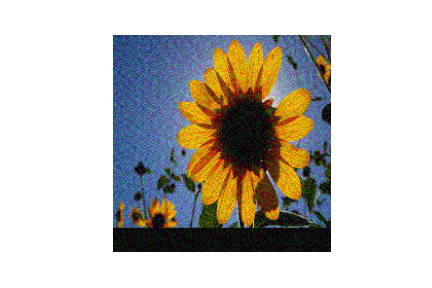
\includegraphics[width=8cm]{images/pr_sunflower_adv_attack_01}
    \end{subfigure}
    \caption{Comparison of adversarial patterns and images generated for NN without pretext training and rotation pretext task}
\end{figure}

\paragraph{Limitations}
\begin{itemize}
    \item Each scenario was recorded only 4 times
    \item Evaluation was done only for 1 dataset
    \item Implementation was not peer-reviewed
    \item Hyper parameters of NN (learning-rate, loss function etc.) were not fine-tuned,
    but just taken as recommended from documentation.
\end{itemize}

\paragraph{Conclusion}
Pretext training did give a little improvement in accuracy as well as robustness against adversarial attacks.
However, it's still far from either competing with pre-training on ImageNet or solving the problem of NNs vulnerability
to adversarial attacks.

